\documentclass[12pt,notitlepage,oneside]{report}
\setcounter{secnumdepth}{3}
\usepackage{neub_cse_thesis}
\usepackage{rotating}
\usepackage{lipsum}
\usepackage{graphicx}
\usepackage{subcaption} 
%\usepackage[acronym, toc]{glossaries}

% Uncomment any of the following lines should you need to
% suppress the LOF, or LOT or LOA

% \suppresslistoffigures 
% \suppresslistoftables
% \suppresslistofalgorithms

% For index creation, comment this out if you do not want to create an index
\makeindex[intoc]
\patchcmd{\titlepage}{empty}{fancy}{}{}
\patchcmd{\chapter}{plain}{fancy}{}{}

\begin{document}   

    % Edit as needed below this line
    % %%%%%%%%%%%%%%%%%%%%%%%%%%%%%%%%%%%%%%%%%%%%%%%%%%%%%%%%
    % Chapter-1
    \chapter{Introduction}\label{intro}
Write your introduction in this section.
Use sections and sub sections to organize the chapters.

\section{Thesis}
The introduction of a thesis serves as a crucial foundation for the research presented. It typically begins by introducing the topic and providing essential background information to contextualize the study. This section outlines the research problem or question, highlighting its significance and relevance within the existing body of knowledge. Additionally, it specifies the objectives of the research, detailing what the study aims to achieve and how it will be conducted. The introduction often concludes with a roadmap that outlines the structure of the thesis, guiding the reader through the upcoming chapters. Overall, the introduction is designed to engage the reader, establish the importance of the research, and clearly articulate the focus and scope of the study.
\section{Project}
The introduction of a project outlines the essential details and context for the work being presented. It typically begins with a brief overview of the project’s topic, followed by background information that situates the project within a broader framework. This section explains the motivation behind the project, including why the chosen theme is significant and what inspired the research. Additionally, it often highlights specific objectives and goals, providing a clear statement of what the project aims to achieve. The introduction may also include a summary of the resources used and the timeline for execution, setting expectations for the reader regarding the project's structure and content. Overall, it serves to engage the audience and establish a foundation for understanding the project's relevance and scope.
\subsection{Subsection}
Sub-subsections are numbered as given above and included as a third level of text. 
\subsubsection{Sub-subsection}
If necessary split your subsections into further sub-subsections.

\section{Guideline for web based projects}
For web based projects, follow the guidelines.
After introductory paragraph go with ther following sections
\begin{itemize}
    \item Project Motivation and Target User Groups
    \item Similar Products and their features
    \item Features of our product as Requirements:
\end{itemize}

\section{Project Motivation and Target User Groups}
First paragraph: Write why did you choose this project.

Second paragraph: Write who will use this project. How will they be benefit using your project.

\section{Similar Products and their features}
Write an introductory paragraph first. In this section you will create several subsections, each outlining one product and its features.
\subsection{Similar Product 1}
Write description of this product in a single paragraph. 

\subsection{Similar Product 2}
Write description of this product in a single paragraph. 
You can also use photographs of some products if you like. An example of how you can add screenshots of similar products is given below:
\begin{figure}[h]
    \centering
    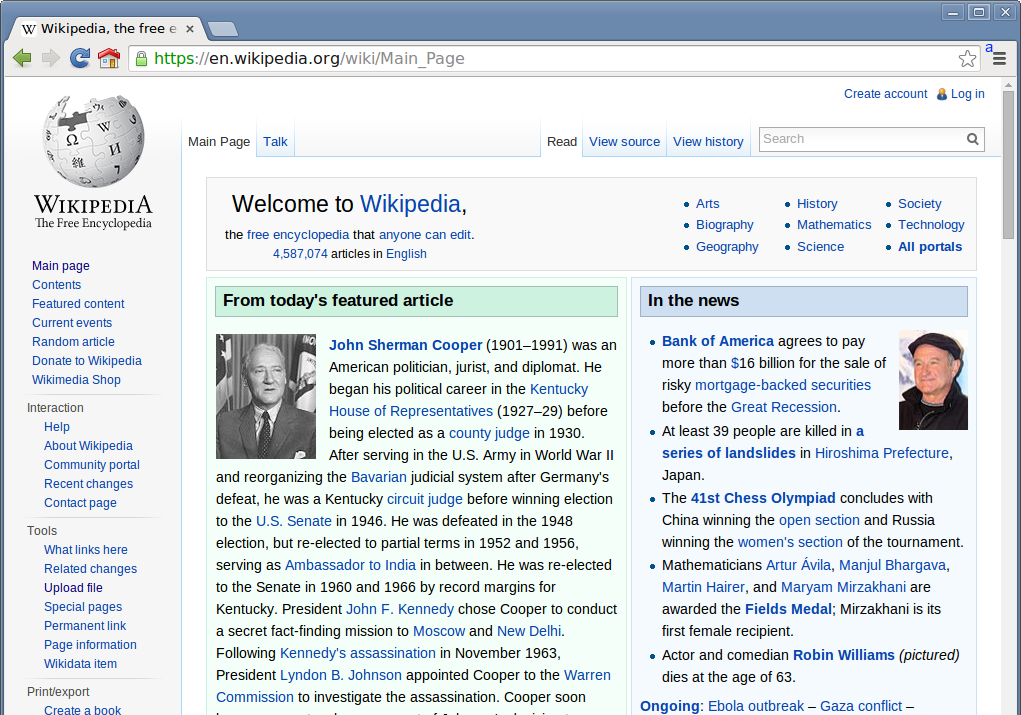
\includegraphics[width=0.7\textwidth]{figures/demoFigure1.png}
    \caption{A sample Wikipedia page.}
    \label{fig:wikiDemo}
\end{figure}
Formatting figures: Always keep the figures center and avoid overstretching the figures. Ideally figures should encompass less that 70\% of text width. 
All figures should be accompanied by relevant caption. Also, all figures must be referenced withing the text. For example the figure \ref{fig:wikiDemo} is a demo page of Wikipedia.
When giving screenshot of others product or using figures of others, you MUST provide proper citation.

\subsection{Similar Product 3}
you have more similar products, add them here.

\subsection{Similar Product 4}
you have more similar products, add them here.


\section{Features of our product as Requirements:}
In this section include both functional and non-functional requirements of your product.

\subsection{Functional Requirement:}
Write all functional requirements as a list.

\subsection{Non-functional Requirement:}
Write all non-functional requirements as a list.

Note that, you will have a separate chapter for requirement analysis. However, you should include a summary of product requirements in the introduction chapter itself.
    
    % Chapter-2
    \chapter{Literature Review}\label{literature_review}
Write your Literature Review in this section.

\section{Section}
Subsections are numbered as given above and included as a second level of text. Text must have the justified alignment. 
Add necessary citation ~\cite{Arora_15}.
\subsection{Subsection}
Sub-subsections are numbered as given above and included as a third level of text. Text must have the justified alignment.
\subsubsection{Sub-subsection}
If necessary split your subsections into further sub-subsections.


\lipsum[3-5]
    
    
    % Chapter-3
    \chapter{Methodology}\label{methodology}

This chapter outlines the research design, data collection methods, and analytical techniques employed in this study. The methodology is designed to ensure that the research objectives are met and that the findings are reliable and valid.


\section{Dataset Acquisition}

In this section explain how dataset used in the study has been acquired. If you have acquired the dataset from any repository link to that repository must be added and also provided in the citation section. Provide \href{https://example.com/record/2000}{\textcolor{blue}{hyperlink}} if necessary. 

Also, provide a slight description of the dataset and mention any data collection that is ongoing and what specific method you are using to collect the data.


\section{Dataset Details}

Provide details about your dataset. You can also provide a snapshot of sample data here to better explain your dataset.

Split your explanation into multiple subsection if necessary.


\subsection{Data Type 1}

Explanation of data type 1. Provide figure if necessary

\begin{figure}[htb ]
    \centering
    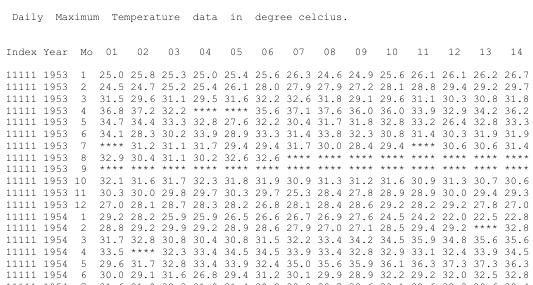
\includegraphics[width=.75\textwidth]{figures/demoFigure2.png}
    \caption{Demo Data Screenshot}
    \label{fig:dataDemo}
\end{figure}

\subsection{Data Type 2}
Explanation of data type 2. Provide tables and figures if necessary

You can write table here like this \ref{tab:numerical_data}.
\begin{table}[h]
    \centering
    \caption{Summary of Numerical Data}
    \label{tab:numerical_data} 
    \begin{tabular}{|c|c|c|c|}
        \hline
        \textbf{ID} & \textbf{Value 1} & \textbf{Value 2} & \textbf{Total} \\ 
        \hline
        1 & 10 & 15 & 25 \\ 
        2 & 20 & 25 & 45 \\ 
        3 & 30 & 35 & 65 \\ 
        4 & 40 & 45 & 85 \\ 
        \hline
    \end{tabular}
\end{table}

You can also include table from external file like \ref{tab:sampleTable}
% Include the table from the external file
\begin{table}[ht]
    \centering
    \caption{Sample Table}
    \label{tab:sampleTable}
    \begin{tabular}{|c|c|c|}
        \hline
        Column 1 & Column 2 & Column 3 \\
        \hline
        Data 1 & Data 2 & Data 3 \\
        Data 4 & Data 5 & Data 6 \\
        \hline
    \end{tabular}
\end{table}


\section{Data Preprocessing}

Explain all the preprossessing done to the dataset in this section. Explain each preprocessing step in individual subsections.

\subsection{Preprocessing 1}
Explain Preprocessing step 1.


\subsection{Preprocessing 2}
Explain Preprocessing step 2.



\section{Dataset insights}
Explain the insight found after the initial preprocessing of the dataset.
\subsection{Correlation Matrix}

\subsection{Insight 2}

\section{Primary training}
Explain how you initially trained your model including all the algorithms used. Provide details about each algorithms.



\section{Data Refinement}
Explain any refinements done in the dataset or preprocessing of dataset done to improve your outcome.


\subsection{Refinement 1}

\subsection{Refinement 2} 


\newpage


\section{Secondary/Final Training}
Explain your final training steps here.

\section{Final Model}
Explain your final model here. You should provide necessary figures to explain your model. All figures should be clear and readable. If necessary you can add figures from PDF files. 

\begin{figure}[h]
    \centering
    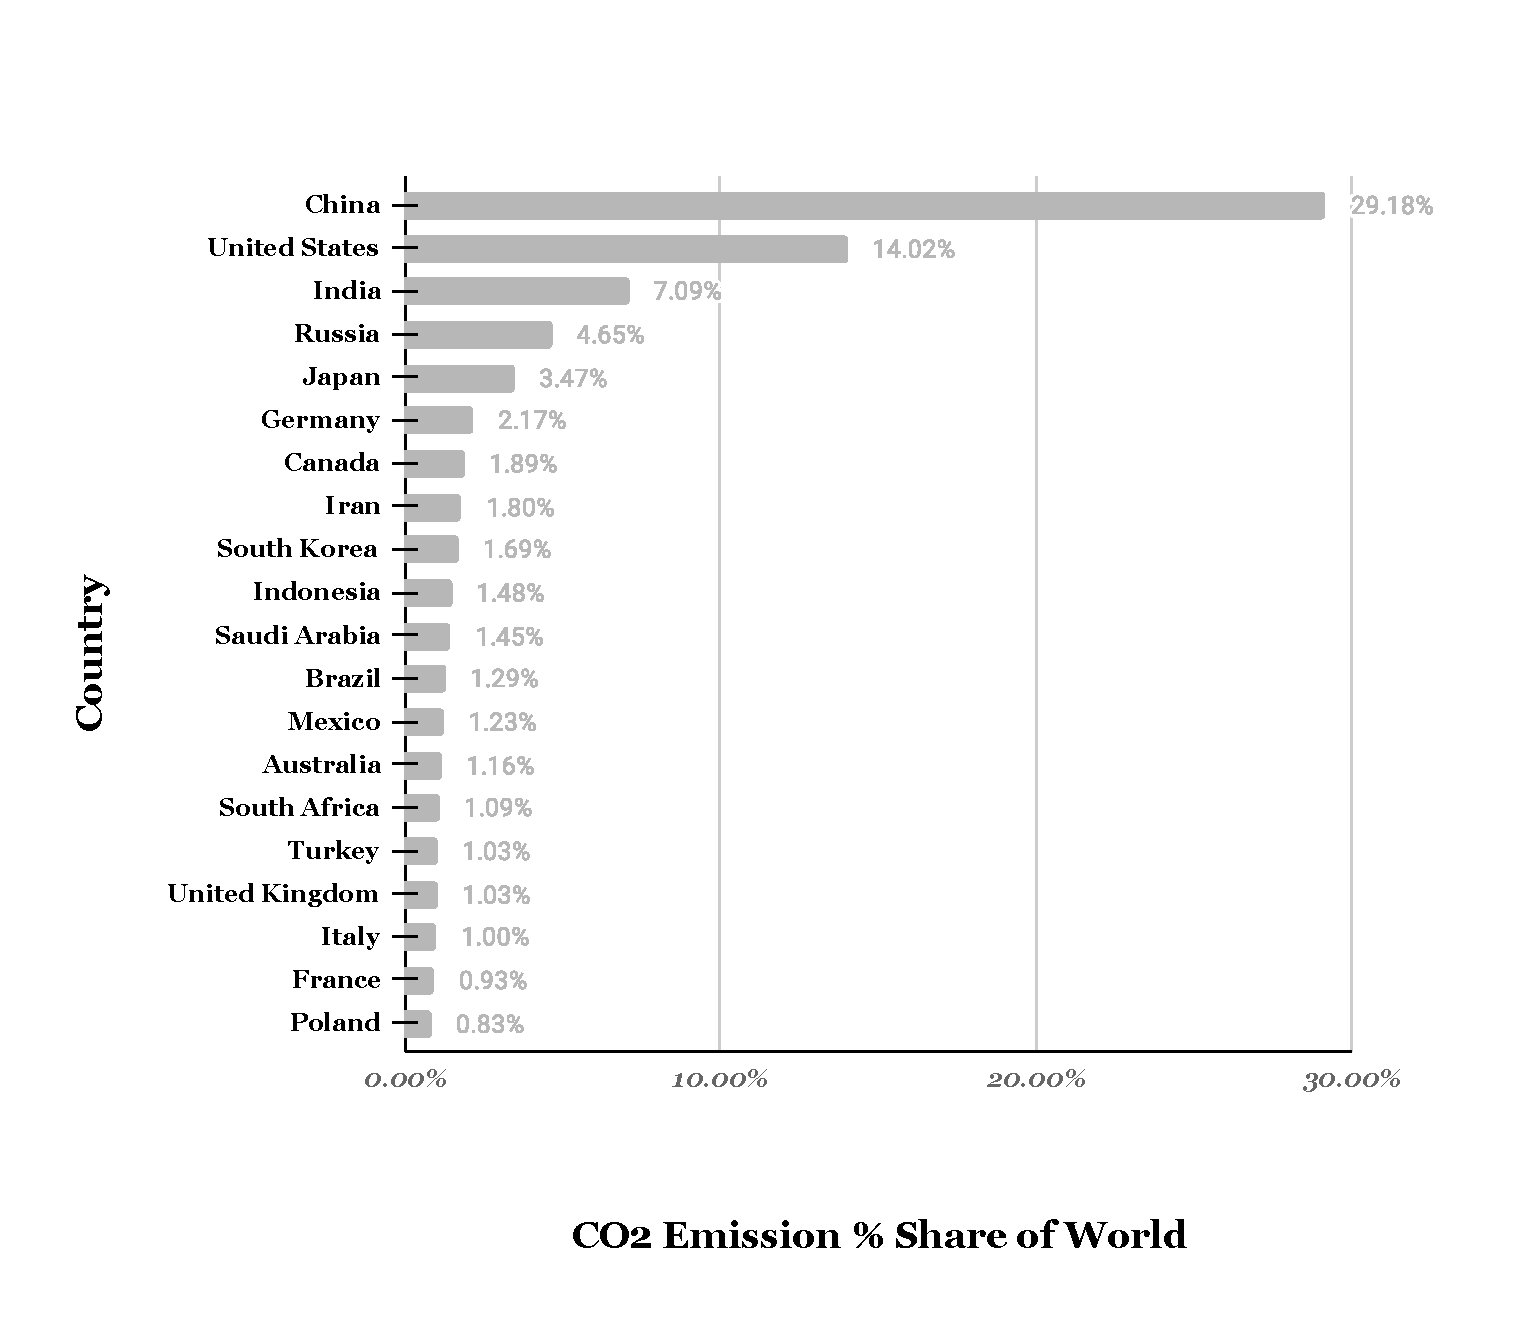
\includegraphics[width=.75\textwidth]{figures/demoFigure3.pdf}
    \caption{Demo Chart}
    \label{fig:dataChart}
\end{figure}



\section{Ethical Considerations}

Provide any ethical considerations you took for your studies and any approval from  Institutional Review Board (IRB).

\section{Limitations}

What are some limitations of your study? Explain it here.
    
    % Chapter-4
    \chapter{Results and Discussion}\label{Results and Discussion}
Write your results and discussion section in here. Split your discussion into multiple sections and subsections as necessary.
\section{Result}
Add nesessary tables and figures to explain your findings.

\begin{table}[ht]
    \centering
    \caption{Result Table}
    \label{tab:resultTable}
    \begin{tabular}{|c|c|c|}
        \hline
        Column 1 & Column 2 & Column 3 \\
        \hline
        Data 1 & Data 2 & Data 3 \\
        Data 4 & Data 5 & Data 6 \\
        \hline
    \end{tabular}
\end{table}

\begin{figure}[h]
    \centering
    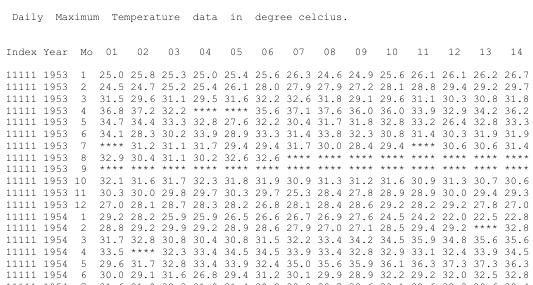
\includegraphics[width=.75\textwidth]{figures/demoFigure2.png}
    \caption{Demo Data Screenshot}
    \label{fig:dataDemo2}
\end{figure}

\section{Discussion}

Add your discussions here. 

Also, make more necessary sections and subsections.

\lipsum[3-15]
    
    % Chapter-5
    \chapter{Conclusion}\label{conclusion}
Place your conclusions here.

\section{Conclusions}

\lipsum[23-25]

\section{Future Prospects of Our Work}

\lipsum[33-35]
    
    % Bibliographies and appendices
    % You do not need to change anything in this file. If you want to
% change the reference style, comment/uncomment the \bibliographystyle
% lines

\clearpage
\renewcommand\bibname{References}
\addcontentsline{toc}{chapter}{\textbf{References}}

% Comment/uncomment as suits you
 \bibliographystyle{IEEEtran} %% IEEE transaction style
% \bibliographystyle{acm} %% ACM style
% \bibliographystyle{alpha}


%\bibliography{chapter/references}
%\bibliography{pages/references}
%\addbibresource{neub_cse_thesis.bib}
\bibliography{neub_cse_thesis}
\endinput

    
    %Uncomment the following line to add appendix. Add more appendix if necessary
    \clearpage
 \begingroup
	\begin{center}
		\textbf{{\Large\Large APPENDIX A}}
	\end{center}
	\addcontentsline{toc}{chapter}{\textbf{APPENDIX A}}
 \label{APPENDIX A}


\textbf{Titile:} Prioritizing the Sustainability Indicators for Applying Artificial Intelligence in Healthcare Decision Making.



Please fill up the following information:
\begin{itemize}
    \item \textbf{Name:}
    \item \textbf{Occupation:}
    \item \textbf{Designation and Organization:}
    \item \textbf{Email:}
\end{itemize}

\lipsum[13-15]

\endinput
\endgroup 
    \renewcommand\leftmark{Appendices}
    
    % Algorithms
    \clearpage
 \begingroup
	\begin{center}
		\textbf{{\Large\Large Algorithms}}
	\end{center}
	\addcontentsline{toc}{chapter}{\textbf{Algorithms}}


\input{algorithms/testAlgorithm.alg}

This algorithm calculates the factorial of a given number \( n \) by iterating from 1 to \( n \) and multiplying each integer together.

\input{algorithms/algorithm2.alg}
This is a test algorithm.

\lipsum[3-5]

\endinput
\endgroup

    
    % Chapter showing example of index creation
    %\chapter{Index Creation}
\section{BUET}
Bangladesh University of Engineering and Technology, abbreviated as
BUET\index{BUET}, is one of the most prestigious institutions for
higher studies in the country. About 5500 students are pursuing
undergraduate\index{BUET!undergraduate} and
postgraduate\index{BUET!postgraduate} studies in engineering,
architecture, planning and science in this institution. At present,
BUET has sixteen teaching departments under five faculties and it has
three institutes. Every year the intake of undergraduate students is
around 900, while the intake of graduate students in Master's and PhD
programs is around 1000. A total of about five hundred teachers are
teaching in these departments and institutes. There are additional
teaching posts like Dr.\ Rashid Professor, Professor Emeritus and
Supernumerary Professors.
 
\section{Campus}
The BUET campus is in the heart of Dhaka\index{Dhaka} --- the capital
city of Bangladesh. It has a compact campus with halls of residence
within walking distances of the academic buildings. The physical
expansion of the University over the last three decades has been
impressive with construction of new academic buildings,
auditorium\index{BUET!auditorium} complex, halls of residence, etc.
 
\section{History}\index{BUET!History}
BUET is the oldest institution for the study of Engineering and
Architecture in Bangladesh. The history of this institution dates back
to the days of Dhaka Survey School which was established at
Nalgola\index{Nalgola}, in Old Dhaka in 1876 to train Surveyors for
the then Government of Bengal of British India. As the years passed,
the Survey School became the Ahsanullah School of
Engineering\index{Ahsanullah School of Engineering} offering
three-year diploma courses in Civil, Electrical and Mechanical
Engineering. In recognition of the generous financial contribution
from the then Nawab of Dhaka, it was named after his father Khawja
Ahsanullah. It moved to its present premises in 1912. In 1947, the
School was upgraded to Ahsanullah Engineering College as a Faculty of
Engineering under the University of Dhaka, offering four-year
bachelor’s courses in Civil, Electrical, Mechanical, Chemical and
Metallurgical Engineering. In order to create facilities for
postgraduate studies and research, Ahsanullah Engineering College was
upgraded to the status of a University in 1962 and was named East
Pakistan University of Engineering and Technology. After the War of
Liberation in 1971\index{1971|see {War of Liberation}}\index{War of
  Liberation}, Bangladesh became an independent state and the
university was renamed as the Bangladesh University of Engineering and
Technology.
 
\section{Students}
Till today, it has produced around 25,000 graduates in different
branches of engineering and architecture, and has established a good
reputation all over the world for the quality of its graduates, many
of whom have excelled in their profession in different parts of the
globe. It was able to attract students from countries like
India\index{India}, Nepal\index{Nepal}, Iran\index{Iran},
Jordan\index{Jordan}, Malaysia\index{Malaysia}, Sri Lanka\index{Sri
  Lanka}, Pakistan\index{Pakistan} and Palestine\index{Palestine}.
 
\section{Departments}
Both Undergraduate and Postgraduate studies and research are now among
the primary functions of the University. Eleven departments under five
faculties offer Bachelor Degrees, while most of the departments and
institutes offer Master's Degrees and some of the departments have
Ph.D. programs. In addition to its own research programs, the
university undertakes research programs sponsored by outside
organizations like European Union, UNO,
Commonwealth\index{Commonwealth}, UGC\index{UGC}, etc. The expertise
of the University teachers and the laboratory facilities of the
University are also utilized to solve problems and to provide
up-to-date engineering and technological knowledge to the various
organizations of the country.


\endinput
    % Index, comment this out if you do not want to create an index
    %\printindex
\end{document}